\documentclass{report}

\usepackage[utf8]{inputenc}
\usepackage[T1]{fontenc}
\usepackage{mathtools}
\usepackage[thinc]{esdiff}
\usepackage{amsmath}
\usepackage{graphicx}
\usepackage{stackengine}


\begin{document}
\setcounter{chapter}{1}
\chapter{Transformations And Expectations}

\section{}
(a) Y = X{\textsuperscript{3}} , f{\textsubscript{X}}(x) = {$42x^{5}(1-x)$}, 0 < x < 1, 
{$g^{-1}(y) = X^{\frac{1}{3}}$}
{$f_{y} = 42x^{\frac{5}{3}}(1 - x{\frac{1}{3}})$} * {$\frac{-1}{3}x{\frac{-4}{3}}$}, On integration it comes to 1
{\newline}
(b) {$g^{-1}(y)$ = {$\frac{Y-3}{4}$}}, {$f_{X}(x) = 7e^{-7x}$} {$\Rightarrow$} {$f_{y} = 7e^{-7{\frac{y-3}{4}}}$} {\textit{Y}} = (3 < y < {$\infty$})
{\newline}
(c) Y = X{\textsuperscript{2}}, f{\textsubscript{{\textit{X}}}(x)} = 30{$x^{2}(1-x)^{2}$}, 0 < x < 1
{$g^{-1}(y) = X^{\frac{1}{2}}$}
{$f_{y} = 20x(1 - x{\frac{1}{2}})$} * {$\frac{-1}{2}{x{\frac{-3}{2}}}$}, On integration it comes to 1
{\newline}

\section{}
(a) Y = {$X^{2}$} {$\Rightarrow$} {$g^{-1}$}(x) = {$x^{\frac{1}{2}}$}
{$f_{y} = \frac{1}{2}x^{\frac{-1}{2}}$}
{\newline}
(b) Y = -log(X) {$\Rightarrow$} {$g^{-1}$}(x) = {$e^{-x}$} {$\Rightarrow$} {$\frac{(n+m+1)!}{n!m!}e^{-xn}(1-e^{-x})^{m} * (-e^{-x}) $}
{\newline}
(c) Y = {$e^x$} {$\Rightarrow$} {$f_{y} = \frac{1}{\sigma^{2}}x^{\frac{-(log y/\sigma)^{2}}{2}}$} * {$\frac{log y}{y}$}
{\newline}

\section{}
{$f_{X}(x) = {\frac{1}{3}}({\frac{2}{3}})^{x}$} {$\Rightarrow$} {$f_{X}(y) = {\frac{1}{3}}({\frac{2}{3}})^{\frac{y}{1-y}}$} {\textit{Y}} {$\rightarrow$} \{0, {$\frac{1}{2}$}, {$\frac{2}{3}$} ... \}

\section{}
(a) f(x) = $\begin{cases} 
	{\frac{1}{2}}{\lambda}{e^{-\lambda x}}  for x {\ge} 0\\
	\\
	{\frac{1}{2}}{\lambda}{e^{\lambda x}}  for x {\le} 0
\end{cases}$
{\newline}
{\newline}
{$\int_{-\infty}^{0}{\frac{1}{2}}{\lambda}{e^{-\lambda x}} + \int_{0}^{\infty}{\frac{1}{2}}{\lambda}{e^{\lambda x}}$} = {$\frac{1}{2}$} + {$\frac{1}{2}$} = 1
{\newline}
(b) {$\int_{-\infty}^{t}{\frac{1}{2}}{\lambda}{e^{-\lambda x}} + \int_{t}^{\infty}{\frac{1}{2}}{\lambda}{e^{\lambda x}}$} = {$\frac{t}{2}$}
{\newline}
f(x) = $\begin{cases} 
	{\frac{1}{2}}{\lambda}{e^{\lambda t}}{ for  {t} \ge}  0\\
	\\
	1 - {\frac{1}{2}}{\lambda}{e^{-\lambda t}}{ for t \le}  0
\end{cases}$
{\newline}
(c) P(|X|< t) = 0 for t {$\le$} 0 and 1 - {$e^{-\lambda t}$} for t > 0
{\newline}

\section{}
answer = {$\frac{1}{\pi}$}{$\frac{1}{\sqrt{Y(1-Y)^2}}$}
{\newline}

\section{}
(a) {$f_{y} = \frac{1}{2}e^{-|Y|^{\frac{1}{3}}} \frac{1}{3}Y^{\frac{-2}{3}}$}
{\newline}
(b) {$f_{Y}(y) = \frac{3}{8}(1-y)^{\frac{-1}{2}} + \frac{3}{8}(1-y)^{\frac{1}{2}}$}, 0 < y < 1
{\newline}
(c) {$f_{Y}(y) = \frac{3}{16}(1 - (1-y)^{\frac{1}{2}})^{2}(1-y)^{\frac{-1}{2}}+ \frac{3}{8}(2 - y)^2$}
{\newline}

\section{}
(a),(b) {$f_{y}(y)$} = $\begin{cases} 
	\frac{2}{9}\frac{1}{\sqrt{y}} \quad \text{  if  } y < 1\\
	\frac{1}{9} + \frac{1}{9}\frac{1}{\sqrt{y}} \quad \text{  if  } y \ge 1\\
\end{cases}$
{\newline}

\section{}
(a) {$F_{x}^{-1}(y) = -ln(1-y)$}
{\newline}
(b) {$F_{x}^{-1}(y)$} = $\begin{cases} 
	ln2y \quad 0 < y < \frac{1}{2}\\
	\frac{1}{2} \quad y = \frac{1}{2}\\
	1 - ln(2 - 2y) \quad 0 < y < \frac{1}{2}\\
\end{cases}$ 
{\newline}
(c) {$F_{x}^{-1}(y)$} = $\begin{cases} 
	ln4y \quad 0 < y \le \frac{1}{4}\\
	-ln(4 - 4y) \quad \frac{3}{4} < y < 1\\
\end{cases}$ 
{\newline}

\section{}
Logically cdf {$F_{x}(x)$} $\sim$ Uniform(0,1)
{$F_{x}^{-1}(x)$} = $\begin{cases} 
	0 \quad \quad -\infty < x \le 1\\
	\frac{(x-1)^{2}}{4} \quad \quad 1 < x < 3\\
	1 \quad \quad 3 \le \infty\\
\end{cases}$ 
{\newline}
\section{}

% TODO: \usepackage{graphicx} required
\begin{figure}
	\centering
	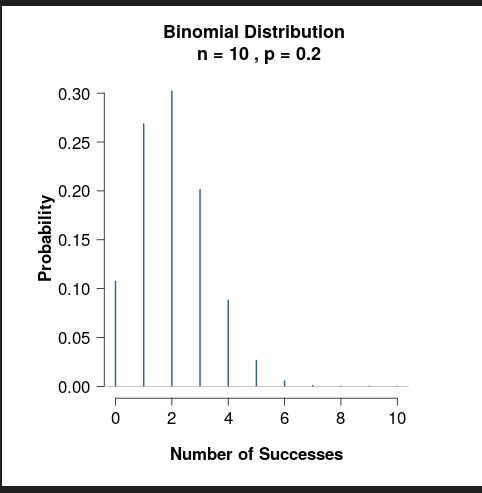
\includegraphics[width=0.7\linewidth]{screenshot001}
	\caption{}
	\label{fig:screenshot001}
\end{figure}

Refer to figure 2.1
{\newline}
logically P(Y > y) $\ge$ P([\textit{U} > y])
{\newline}
P(Y < y) $\le$ P([\textit{U} < y])
{\newline}
for some x = x{\textsubscript{0}}
P(Y > y) = P([\textit{U} > y])
but at next point {$\epsilon$}, P(Y > y) will be stagnant since its a discrete probability. But P([\textit{U} > y]) will eventually be lifted some points up. So the two cases are justified

\section{}
(a) {$\textit{f}_{\textit{X}}$}(x) = {$\frac{1}{\sqrt{2\pi}}$}e{\textsuperscript{-x{\textsuperscript{2}/2}}}
{\newline}
{$\int_{-\infty}^{\infty}x^{2}$}{$\frac{1}{\sqrt{2\pi}}$}e{\textsuperscript{-x{\textsuperscript{2}/2}}}dx
{\newline} {$\Rightarrow$} Y = X{\textsuperscript{2}}

{$f_{y}(y) = 2(\frac{1}{\sqrt{2\pi}}e^{-\frac{x^{2}}{2}}|\frac{1}{\sqrt{2\pi y}}|)$}

Integrating gives 1
{\newline}
(b){$\textit{f}_{\textit{X}}$}(x) = {$\frac{1}{\sqrt{2\pi}}$}e{\textsuperscript{-x{\textsuperscript{2}/2}}}
EY = {$\frac{2}{\pi}$}
EY{\textsubscript{2}} = 1
{\newline}
(EY) = 1 - {$\frac{2}{\pi}$}
\section{}
skipping

\section{}
{$\textit{f}_{\textit{X}}(X) = $} = p(1-p){$\textsuperscript{x}$} + (1-p)p{$\textsuperscript{x}$}
{\newline}
EX = p(1-p)[$\frac{1}{p^{2}} + \frac{1}{(1-p)^{2}}$]
{\newline}

\section{}
(doubt) EX = {$\int_{0}^{\infty}xf_{X}(x)$} Integration by parts
{\newline}
EX = {$\left[xF_{X}(x)\right]_{0}^{\infty} \quad - \quad \int_{0}^{\infty}F_{X}(x)dx$}
Now let say the identity is true
{\newline}
{$\int_{0}^{\infty}[1 - F_{X}(x)]dx = \int_{0}^{\infty}dx \quad - \quad \int_{0}^{\infty}F_{x}(x)dx$} 
{\newline}
So 1{\textsuperscript{st}} term doesn't make any sense
{\newline}


\newcommand{\btimes}{\mathbin{\rotatebox[origin=c]{90}{$<$}}}
\newcommand{\atimes}{\mathbin{\rotatebox[origin=c]{-90}{$<$}}}

\section{}
{$\int_{-\infty}^{\infty}xf_{1}(x)dx + \int_{-\infty}^{\infty}xf_{2}(x)dx = \int_{-\infty}^{\infty}x(f_{1}(x) + f_{2}(x))dx = \int_{-\infty}^{\infty}x(min(f_{1}(x),f_{2}(x)) + max(f_{1}(x),f_{2}(x)))dx$} = (X $\btimes$ Y) + (X $\atimes$ Y) = X + Y
{\newline}
Hence by rearranging we get the equation
{\newline}

\section{}
{$\int_{0}^{\infty}ae^{-\lambda t} + (1-a)e^{-\mu t} = \frac{a}{\lambda} + \frac{1-a}{\mu}$}
{\newline}

\section{}
(a) m = {$2^{\frac{1}{3}}$}
{\newline}
(b) m = 0
{\newline}

\section{}
E|X-a| = {$\int_{-\infty}^{\infty}|x - a|f(x) = \int_{-\infty}^{a}(-x + a)f(x) + \int_{a}^{\infty}(x - a)f(x)$}. On differentiating,
{\newline}
{$\frac{d E|x - a|}{da} = \int_{-\infty}^{a}f(x) - {\int_{a}^{\infty}f(x) = 0} \Rightarrow  \int_{-\infty}^{a}f(x) = \int_{a}^{\infty}f(x)$} 
{\newline}

\section{}
{$E|X-a|^{2} = \int_{-\infty}^{\infty}(x-a)^{2}f(x)dx = \frac{dE}{dx} = \int_{-\infty}^{\infty}2(x-a)f(x)dx \Rightarrow \int_{-\infty}^{\infty}xf(x) = a{\int_{-\infty}^{\infty}f(x)dx} = a(1) \Rightarrow EX = a$}
{\newline}

\section{}
{$EX = {\sum_{k=0}^{k=\infty}k(1-p)^{k}p = \frac{1}{p^{2}}}$}
{\newline}

\section{}
{$Eg(X) = {\int_{-\infty}^{\infty}g(X)f_{X}(x)dx = {\int_{-\infty}^{\infty}yf_{X}(g^{-1}{y})|\frac{dg^{-1}(y)}{dy}|dy = \int_{-\infty}^{\infty}yf_{y}(y)dy = EY}}$}
{\newline}

\section{}
(a) Integration leads to 1.
{\newline}
(b) EX = {$\frac{2\beta}{\sqrt{\pi}}$}, Var(X) = {$\beta^{2}(\frac{3}{2} - \frac{4}{\pi})$}
{\newline}

\section{}
{$f_{y}(y) = \frac{1}{2}y^{\frac{-1}{2}}$}
{\newline}
EY = {$\frac{1}{3}$}
{\newline}
EY{\textsuperscript{2}} = $\frac{1}{5}$
{\newline}
Var(y) = $\frac{4}{45}$
{\newline}

\section{}
(a), (b), (c) same as above
{\newline}

\section{}
Let A = {$\int_{0}^{X}f_{X}(x)dx$}
Now {$\int_{0}^{-X}f_{X}(x)dx \Rightarrow Y = -X \Rightarrow dY = -dX \Rightarrow \int_{-X}^{0}f_{X}(x)dx \Rightarrow -\int_{Y}^{0}f_{Y}(y)dy = A$}
{\newline}
Hence symmetrical
{\newline}

\section{}
{$M_{X}(t) = \int_{-\infty}^{\infty}e^{tx}f_{X}(x)dx$}
{\newline}
{$M_{X}(-t) = \int_{-\infty}^{\infty}e^{-tx}f_{X}(x)dx \Rightarrow \int_{-\infty}^{\infty}e^{t(-x)}f_{X}(-x)dx. Let j = -x {\Rightarrow} dj = -dx -\int_{\infty}^{-\infty}e^{tj}f_{X}(j)dj = M_{x}(t)$}
{\newline}

\section{}
(a) gaussian, |x|, x{\textsuperscript{2}}
{\newline}
(b) {$\int_{-\infty}^{a}f_{X}(x) = \int_{a}^{\infty}f_{X}(x) \Rightarrow x = a-y \Rightarrow \int_{0}^{\infty}f_{X}(a-y)dy = \int_{-\infty}^{a}f_{X}(a-y)dy  \Rightarrow$}a is the median
{\newline}
(c) Wrong sol {$\int_{-\infty}^{\infty}xf_{X}(x)dx = \int_{-\infty}^{a}xf_{X}(x)dx + \int_{a}^{\infty}xf_{X}(x)dx \newline 
	\text{let for first part x} \rightarrow \text{a - x and second part x} \rightarrow x - a \newline
	-\int_{\infty}^{0}((a-x)f_{X}(a-x))dx + \int_{0}^{\infty}((x-a)f_{X}(x-a)dx) = \int_{0}^{\infty}((a-x)f_{X}(a-x))dx + \int_{0}^{\infty}((x-a)f_{X}(x-a)dx) = \int_{0}^{\infty}((a-x)f_{X}(a-x))dx + \int_{0}^{\infty}((x-a)f_{X}(a-x)dx) = 0 \newline \text{symmetric function}
	$}
	{\newline}
(d) It has a monotonic slope. Hence it cant have a symmetric pdf {\newline}
(e) EX = 1, m median = ln2 {\newline}

\section{}
(a) Gaussian distribution {\newline}
(b) uniform distribution {\newline}
(c) Let assume that the point of symmetry is not the modial point. Since the function is symmetric there will be another x for which the mode value will be same. This is in contradiction as our function is unimodal. Hence its symmetric about the mode. {\newline}
(d) for a $\ge$ x $\ge$ y where a = 0 and f(0) $\ge$ x $\ge$ y. {\newline}

\section{}
(a) Let think logically x-a will shift the a{\textsuperscript{th}} to zero. Hence symmetrical. {\newline}
(b) {$\alpha_{3}$} = 2 {\newline}
(c) (i) {$\alpha_{4} = 3$} (ii) {$\alpha_{4} = \frac{9}{5}$} (iii) {$\alpha_{4} = 6$}
{\newline}

\section{}
(a) EX{\textsuperscript{2}} = n(n-1)p{\textsuperscript{2}} + np. EX = np
So E(X(X-1)) = n(n-1)p{\textsuperscript{2}} (binomial)

EX{\textsuperscript{2}} = {$\lambda\textsuperscript{2}$} + {$\lambda$}
EX = {$\lambda$}
E(x(x-1)) = {$\lambda\textsuperscript{2}$}
{\newline}
(b) Var(binomial) = n(n-1)p{\textsuperscript{2}} - np{\textsuperscript{2}}
Var(binomial) = {$\lambda\textsuperscript{2}$} + {$\lambda$} - {$\lambda\textsuperscript{2}$} = $\lambda$
{\newline}
(c) I wont be able to solve
{\newline}

\section{}
(a) M{\textsubscript{X}}(t) = $\frac{e^(tx) - 1}{ct}$
{\newline}
(b) M{\textsubscript{X}}(t) = $\frac{2}{c^2}((c-1)e^c -c + 1)$
{\newline}
(c) M{\textsubscript{X}}(t) = $\frac{4e^{\alpha t}}{4 - \beta^2 t^2}$
{\newline}
(d) P(X = x) = {$\sum_{x=0}^{x=\infty}(\stackanchor{ r + x - 1 }{x})p^{r}(1-p)^{x}dx$} {$\Rightarrow$}
{\newline}
{$M^{X}(t) = \sum_{x=0}^{x=\infty}e^{tx}(\stackanchor{r + x - 1}{x})p^{r}(1 - p)^{x}dx \Rightarrow \sum_{x=0}^{x=\infty}e^{tx}(\stackanchor{r + x - 1}{x})p^{r}((1 - p)e^{t})^{x}(1 - ((1 - p)e^{t}))^{r}dx = 1 {\Rightarrow} M_{X}(t) = (\frac{p}{(1 - ((1 - p)e^{t}))})^{r}$}
{\newline}

\section{}
{$M_{X}(0) = 0, But M_{X}(0) = 1 as the distribution of pmf should be 1. So no$}
{\newline}

\section{}
{$\frac{d}{dt} S(t) = \frac{M_{X}^{'}(t)}{M_{X}(t)} Putting t = 0 we get M_{X}(0) = 1, M_{X}^{'} = EX, \text{Same go by differentiating divide rule and you will get} M_{X}^{''}(t) - (M_{X}^{t})^{2} \Rightarrow EX^{2} - (EX)^{2}$}
{\newline}

\section{}
(a) {$M_{X}(x) \sum_{x=0}^{x=\infty}\frac{e^{tx}e^{-\lambda}\lambda^{x}}{x!} \text{Using Taylor series } e^{-\lambda} * e^{\lambda e^{t}} $} Hence we derive the {$M_{X}(t)$}. (Rest is Maths) EX = $\lambda$ EX{\textsuperscript{2}} = $\lambda^{2} + \lambda$ Var(x) = $\lambda$
{\newline}
(b) {$M_{X}(X) \sum_{x=0}^{x=\infty}p(1-p)_{x}$} (Think in terms of Geometric Mean.) {$M_{X}(t) = \frac{p}{1 - (1-p)e^{t}}$}
{\newline}
EX = $\frac{1-p}{p}$, EX{\textsuperscript{2}} = $\frac{p(1-p) + 2(1 - p )^{2}}{p^2}$ Var(x) = $\frac{1 - p}{p^2}$
{\newline}
(c) Yes its an mgf (Some complicated mathematics) EX = $\mu$  EX{\textsuperscript{2}} = {$\mu^{2}$} + {$\sigma^{2}$}. Var(x) = {$\sigma^{2}$} {\newline}

\section{}
(a) $\int_{\infty}^{\infty}x^{r} * \frac{1}{\sqrt{2\pi}x} * e^{-(log x)^{2}/2} = e^{r^{2}/2}$
{\newline}
(b) $e^{r^2/2 - 2\pi^{2}}$
{\newline}

\section{}
{$\int_{0}^{\infty} \frac{e^{tx}}{\sqrt{2\pi}x}e^{-(log)^2/2}dx 
\newline = \lim_{x \rightarrow \infty}e^{tx - log^{2}(x)} \newline \lim_{x \rightarrow \infty}\frac{e^{tx}}{e^{log^2(x)}} \text{Taking log} \newline = \lim_{x \rightarrow \infty}\frac{tx}{log^2(x)} \text{    On solving} \lim_{x \rightarrow \infty}tx/2 \rightarrow \infty $}
{\newline}

\section{}
(a) \begin{figure}
	\centering
	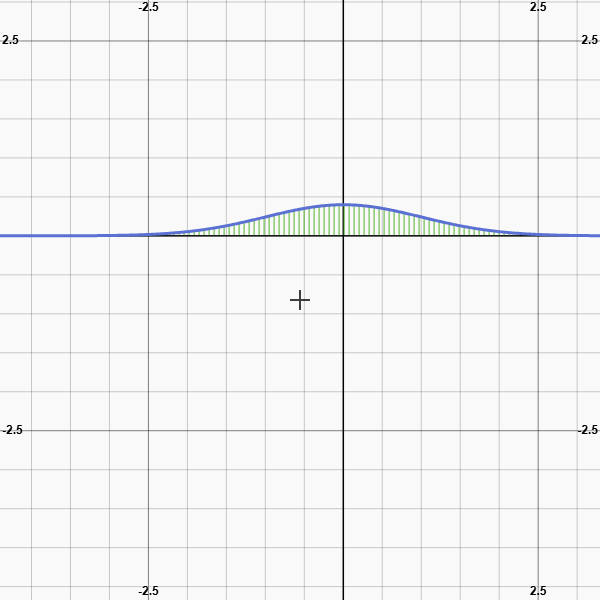
\includegraphics[width=0.7\linewidth]{normal_distribution}
	\caption{}
	\label{fig:normal_distribution}
\end{figure}
\begin{figure}
	\centering
	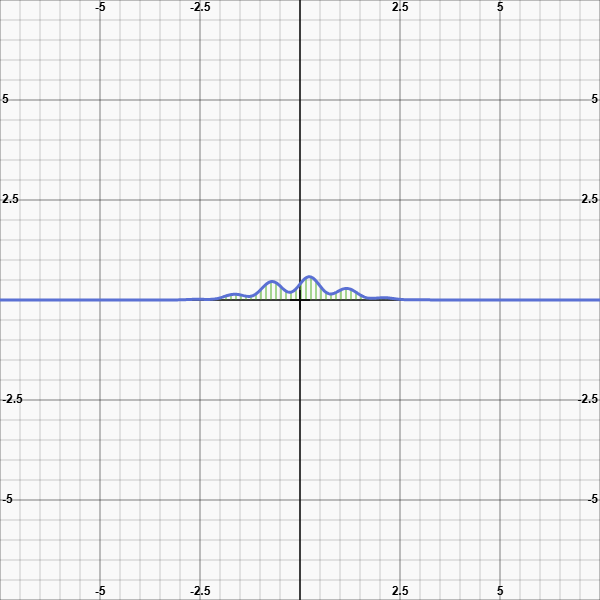
\includegraphics[width=0.7\linewidth]{second_function}
	\caption{}
	\label{fig:second_function}
\end{figure}
{\newline}
(b) \begin{figure}
	\centering
	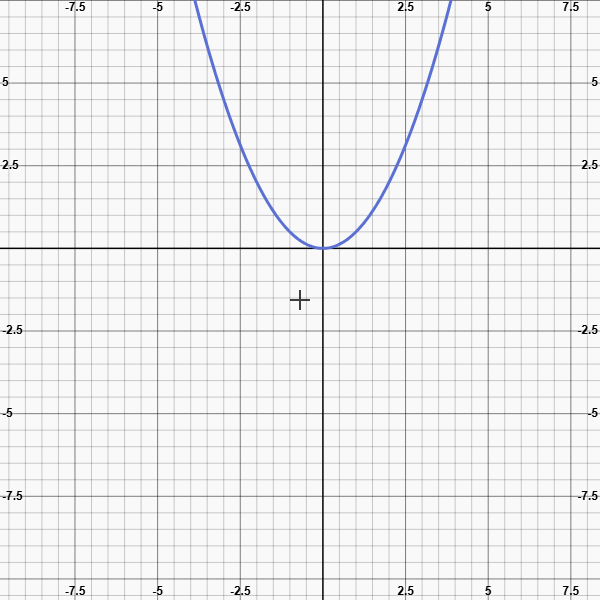
\includegraphics[width=0.7\linewidth]{K1_T}
	\caption{}
	\label{fig:K1_T}
\end{figure}
\begin{figure}
	\centering
	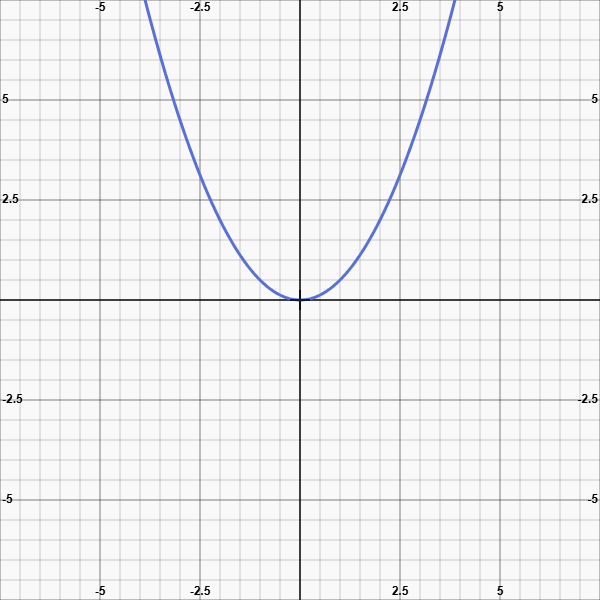
\includegraphics[width=0.7\linewidth]{K2_T}
	\caption{}
	\label{fig:K2_T}
\end{figure}
{\newline}
(c) (i) {$M_{X}(t) = e^{K_{1}}$} {\newline}
{ii} {$M_{X}(t) = e^{K_{2}}$} {\newline}
{\newline}
(d) make transformation e{\textsuperscript{x}} 
{\newline}

\section{}
(a) {$M_{X}(t) = [p/(1 - (1-p)e^t)]^r$}
{\newline}
(b) {$M_{X}(t) = [p/(1 - (1-p)e^2pt)]^r$} On solving $[\frac{1}{1-2t}]^r$
{\newline}

\section{}
(a) {$e^{-\lambda x}$} {\newline}
(b) {$\frac{-1}{\lambda ^ 2}$} {\newline}
(c) {$\frac{-1}{t^2}$} {\newline}
(d) {$\frac{1}{(1-t)^2}$}
{\newline}




















\end{document}